\documentclass{subfiles}

\begin{document}

    \chapter{Implementaciones sobre el sistema de Realidad Aumentada}
    \label{chap:3}

        \section{Modelo en 3D y Three.js}
        \label{sec:3.1}
        A partir del sistema básico generado en el capítulo anterior, podemos empezar a añadirle complejidad a nuestro sistema. El primer elemento que añadiremos es un modelo en 3D que utilizaremos como base en esta aplicación.

        \paragraph{}
        Para la carga, inserción, control y movimientos de los modelos en 3D se ha utilizado en esta aplicación la librería \threejs. \threejs es una librería ligera preparada para su uso en aplicaciones web compatible con \js \cite{web:wikipediathreejs}. Además, este está especializado en el control de modelos en 3D en formato \glb y \gltf, que son dos formatos basados en \textit{JSON} y que están creados para ser óptimos en tiempo de ejecución (el formato \glb es el equivalente en binario a \gltf) \cite{web:threejs_loading3dmodels}.

        \paragraph{}
        La librería \threejs basa su funcionalidad en el uso de Escenas o \textit{Scenes}, el objeto que utiliza esta librería para almacenar y presentar sus modelos en 3D, la iluminación o focos de luz que los alumbrarán y las cámaras virtuales que observarán a estos mismos \cite{web:threejs_scene}. Aplicando un símil sencillo, la Escena de \threejs podría equivaler a una escena de cine, donde los actores equivaldrían a los modelos en 3D, los focos equivaldrían a la iluminación y las cámaras equivaldrían a las cámaras virtuales. Este último concepto es muy importante, debido a que afectará continuamente al renderizado de los modelos en 3D.

        \paragraph{}
        La cámara virtual es la que simula el punto de vista del espectador, ya sea en \ra, en \rv o en otras virtualizaciones que utilicen modelos en 3D como son las simulaciones, los videojuegos o las películas de animación \cite{web:mozilla_virtualcamera}. A alto nivel, una cámara virtual, además de la posición del espectador, definiría también lo que este va a poder observar de manera que, cuando se va a renderizar una imagen, solo tiene que generarse la parte visible de los modelos que entren en el rango de visión de la cámara virtual.

        \begin{figure}
        \centering
        \fbox{
        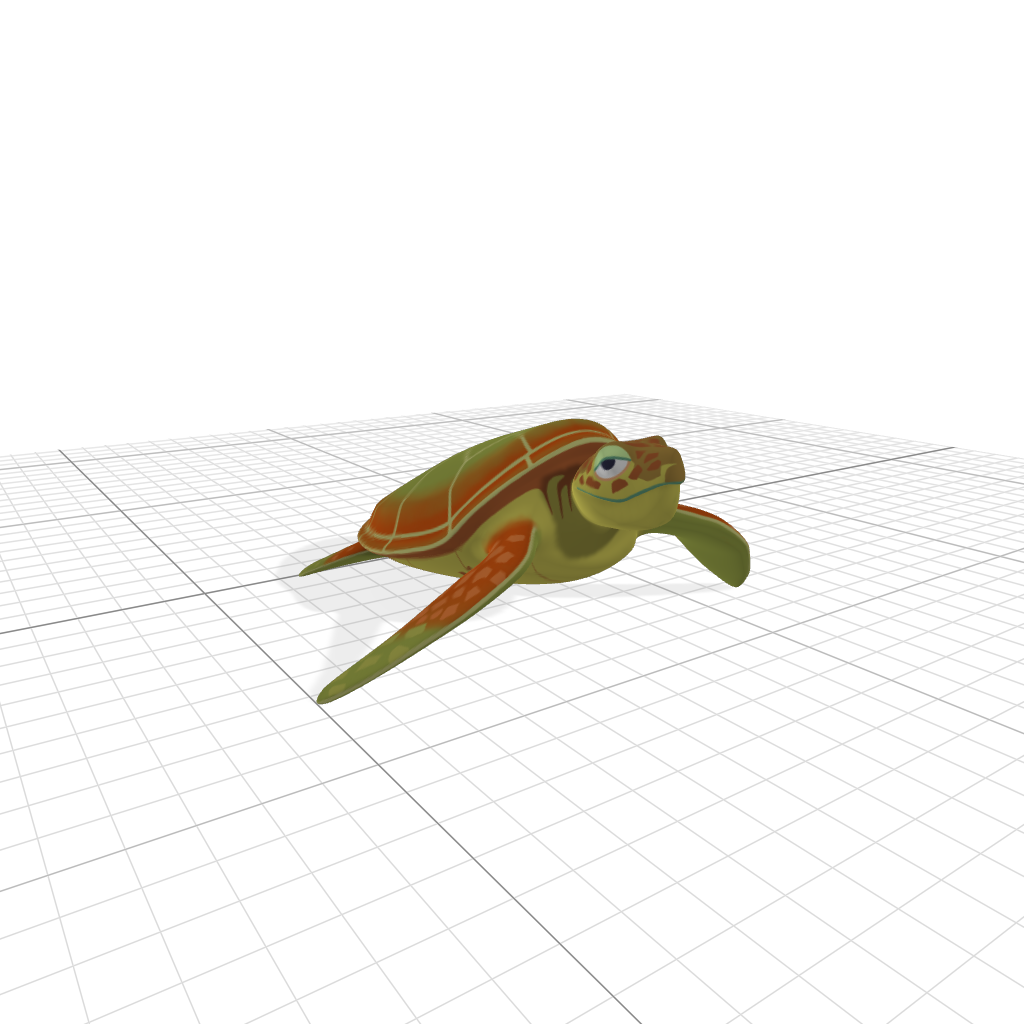
\includegraphics[width=0.6\textwidth]{img/tortuga_marina.png}
        }
        \caption{Ejemplo de renderizado de un modelo en 3D extraído de la biblioteca de modelos 3D de la aplicación de Windows \textit{Visor 3D}.}
        \label{fig:tortuga_marina}
        \end{figure}

        \paragraph{}
        Visualizando esto último con un ejemplo, en la figura \ref{fig:tortuga_marina} se ha renderizado un modelo 3D de una tortuga marina. En este renderizado, la cámara virtual se encuentra frente al modelo, pero ligeramente ladeado hacia la parte derecha de la tortuga. Debido a la posición de la cámara, no es necesario que se renderice la pata izquierda trasera de la figura, puesto que lo tapa el resto del cuerpo. Sin embargo, si la cámara se encontrase detrás de la tortuga, sería necesario renderizar ambas patas traseras y la cola, pero no se renderizaría la cara de la figura. De la misma manera, si la cámara no estuviese apuntando hacia la tortuga, no habría ningún modelo 3D que renderizar.
        
        \paragraph{}
        Aunque este parezca un concepto obvio, es necesario explicarlo, debido a que será necesario establecer la posición y orientación de la cámara virtual durante el desarrollo. Esto es porque la cámara virtual coincidirá con la posición de la cámara del dispositivo móvil. Cuando la cámara apunte hacia una figura en 3D en la \ra, se incrustará en la pantalla del móvil la parte de la figura que se vea desde la cámara virtual (es decir, se debe ver por la pantalla lo que se vería a través de la cámara si esta figura existiese en nuestra Realidad).

        \paragraph{}
        Una vez explicado esto, es necesario volver al código. Siguiendo el orden de carga, el primer lugar donde nos detendremos es en la función \textit{callback} \textit{checkSessionSupported}, vista en la sección \ref{sec:2.2}, que es la función que se lanza desde el constructor del Controlador y que inicializaba los elementos más pesados antes de que el usuario pulsase el botón de iniciar la Sesión de \ra. En esta, ya habíamos visto las acciones que se realizaban en caso de que el navegador no fuese compatible con \webxr, pero ahora vamos a ver algunas de las que se ejecutan en el caso positivo. Ampliando el código \ref{lst:2.2} al que hacemos mención:

\newpage
\begin{lstlisting}[language=JavaScript, caption={Carga de elementos de Three.js si se soporta la sesión.}, label={lst:3.1}]
// Constantes
#RETICLELINK = "http://url_donde_se_aloja_el_modelo_3d";

#checkSessionSupported = (isSupported) => {
    if (isSupported) {
    
        // Scene y Loader
        this.#scene = new THREE.Scene();
        this.#loader = new THREE.GLTFLoader();
        // ...

        // Modelo en 3D: Reticula
        this.#loader.load(this.#RETICLELINK, function(gltf) {
            // Figura
            this.#reticle = gltf.scene;
            this.#reticle.visible = false;
            this.#scene.add(this.#reticle);
        }.bind(this));
        // ...
    
    } else {
    
        document.getElementById("arButton").disabled = true;
        alert("Tu navegador no permite una sesi\xF3n de Realidad Aumentada.");
        
    }
};
\end{lstlisting}

        Aquí ya podemos ver tres elementos de cierto peso que se están cargando previamente antes de iniciar la Sesión: la Escena, una instancia de \textit{GLTFLoader} y, desde una función de esta última, un modelo 3D al que llamaremos a partir de ahora, <<retícula>>, sencillamente porque es el nombre del modelo original alojado en la librería de modelos de ejemplo de \webxr en GitHub. Este modelo en 3D, que podemos ver en la figura \ref{fig:reticle} será el que utilicemos como base para el funcionamiento de esta aplicación, haciendo las veces de <<puntero>> más adelante, cuando queramos señalar un punto en el suelo para ubicar la figura humana que desarrollemos.

        \begin{figure}
        \centering
        \fbox{
        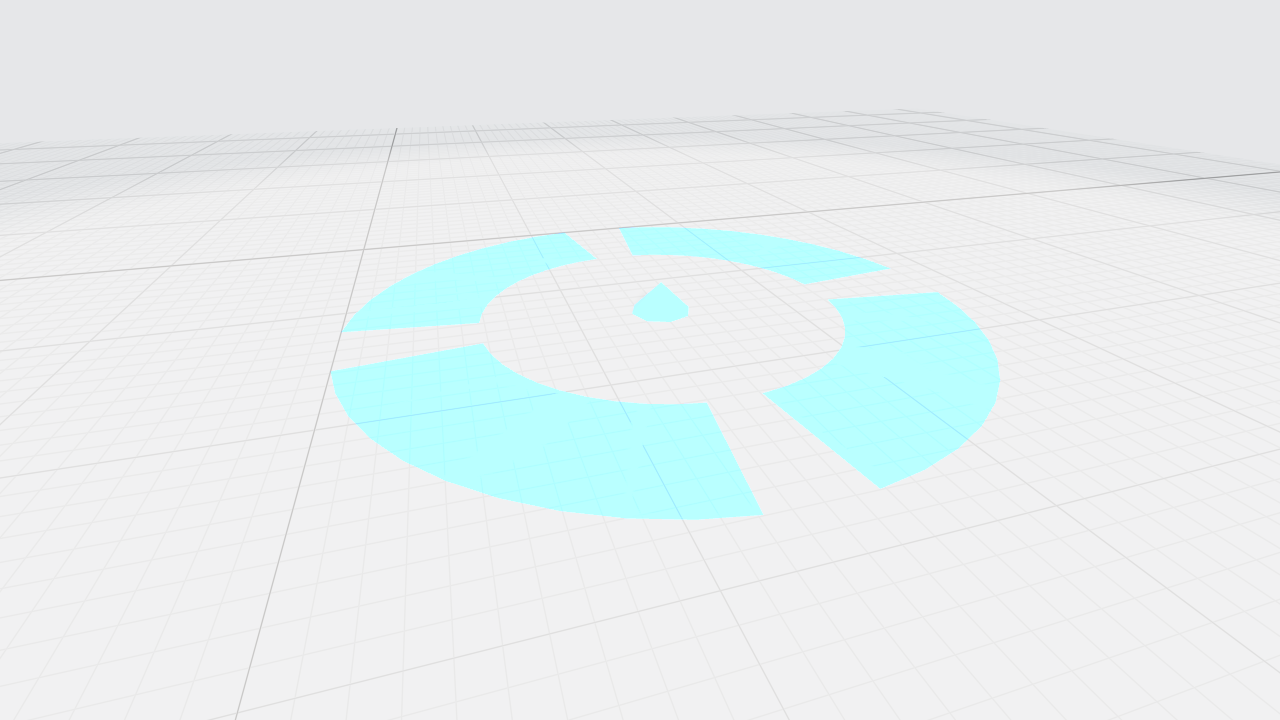
\includegraphics[width=0.6\textwidth]{img/reticle.png}
        }
        \caption{Muestra de la Retícula utilizada en esta aplicación. Modelo obtenido del repositorio \textit{webxr} del perfil de \textit{Immersive Web at W3C}, en GitHub.}
        \label{fig:reticle}
        \end{figure}

        \paragraph{}
        En primer lugar, inicializamos la Escena en la línea 8 para poder introducir la retícula más adelante (volviendo al símil anteriormente utilizado, es como si el actor <<retícula>> entrara en escena). Sin embargo, esto no lo podemos hacer hasta que se haya cargado el modelo. Para esto, utilizamos el objeto \textit{loader}.
        
        %% carga de figuras
        %% ubicacion de las figuras

        \section{Cálculo de superficies, \textit{Hit Test Results}}
        \label{sec:3.x}

        \section{Animación de modelos}
        \label{sec:3.y}
        %% clock
        %% comentar también el evento onTouch

        \section{Sonido espacial}
        \label{sec:3.z}
        %% comentar tambien el evento onsessionend

        \section{Funcionamiento final de la Realidad Aumentada}
        \label{sec:3.a}
        %% 
        %% carga aleatoria de figuras
        %% sustitucion de reticula por figuras

        

\end{document}